
\chapter{Obrazowanie wielospektralne}
Obrazowanie wielospektralne jest techniką rejestracji obrazu za pomocą fal elektromagnetycznych o~wybranej częstotliwości spośród widma spektroskopowego. Podczas gdy ludzkie oko widzi głównie w trzech zakresach spektralnych (czerwonym, niebieskim oraz żółtym), obraz wielospektralny jest rejestrowany w znacznie większej liczbie zakresów (przykładowo 31).

\section{Format danych}
\index{kostka wielospektralna} Dane wielospektralne są często nazywane kostką wielospektralną. 

\begin{figure}[ht]
	\centering
		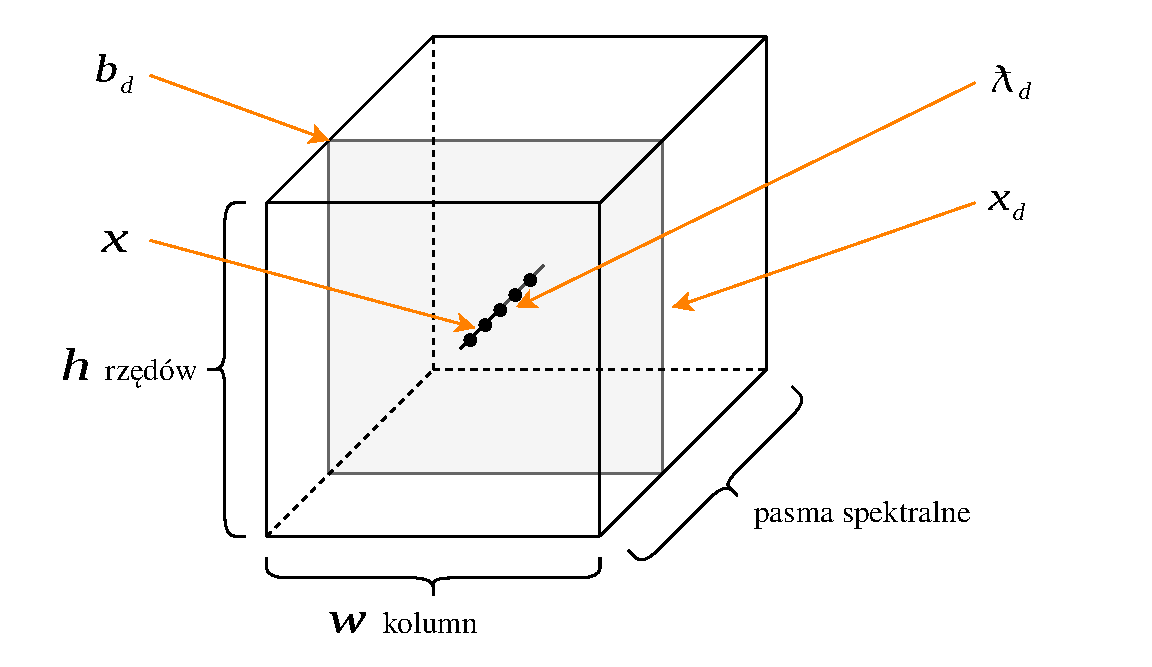
\includegraphics[width=0.75\linewidth]{rys02/multispectral-cube-vector}
	\caption{Schemat kostki wielospektralnego}
	\label{fig:multispectral-cube}	
\end{figure}

Na rysunku ~\ref{fig:multispectral-cube} zilustrowano układ danych w kostce wielospektralnej. Kostka taka składa się z~$n_x$ ($h$ rzędów na $w$ kolumn) pikseli $x$. Każdy piksel jest wektorem współczynników spektralnych o~długości  $n_D$, gdzie $n_D$ jest liczbą obrazów spektralnych, na które składa się dana wielospektralna. Każdy współczynnik $x_d$ jest wartością reakcji sensorycznej dla odpowiadającego pasma spektralnego $b_d$ skoncentrowanego wokół fali $\lambda_d$. W skrócie obraz wielospektralny jest zbiorem obrazów rejestrowanych przy użyciu fal elektromagnetycznych o~zadanych długościach. 


\subsection{Konsekwencje formatu danych}
Ze względu na swoją charakterystykę serie obrazów wielospektralnych mogą bezproblemowo osiągać rozmiary setek megabajtów, lub nawet gigabajtów. Zazwyczaj jednak obrazy są rejestrowane aparatem o~matrycy ok. 2 Mpix. Większość danych pochodnych, które są efektem analizy tego obrazu posiadają podobne rozmiary. Informacja ta jest kluczowa podczas projektowania mechanizmu zarządzania danymi w~takim systemie. Biorąc pod uwagę rozmiar danych mechanizm taki powinien:
\begin{itemize}
\item unikać tworzenia zbędnych kopi danych,
\item dokonywać obliczeń danych wyłącznie na żądanie,
\item zwalniać z~pamięci dane, które nie są już wykorzystywane przez aplikację.
\end{itemize}

\section{Dane w systemie Gerbil}

Oryginalny obraz wielospektralny jest traktowany jako dana wejściowa w systemie. Na jego podstawie powstają dane pochodne. Są to głównie kolejne obrazy oraz histogramy wielospektralne. Do stworzenia prototypu mechanizmu zarządzania danymi oraz procesem przetworzenia użyte zostały poniższe dane:
\begin{itemize}
	\item \index{image} \textbf{image} -- oryginalny obraz wielospektralny. Dana ta jest obliczana podczas inicjalizacji aplikacji. Użytkownik może wejść w interakcję z~systemem dopiero gdy image zostanie przetworzone.
	\item \index{ROI} \textbf{ROI (Region of Interest)} -- wyselekcjonowany podzbiór danych, w tym przypadku wybrane prostokątne zaznaczenie obrazu. Jest przechowywany jako współrzędne lewego górnego wierzchołka zaznaczenia, jego wysokość oraz szerokość,
	\item \index{image.IMG} \textbf{image.IMG} -- fragment obrazu oryginalnego zdeterminowany przez ROI,
	\item \index{image.NORM} \textbf{image.NORM} -- image.IMG po normalizacji wektorów składających się z~pikseli o~jednakowych współrzędnych na przestrzeni pasm spektralnych,
	\item \index{image.GRAD} \textbf{image.GRAD} -- gradient obrazu image.IMG,
	\item \index{image.PCA} \textbf{image.PCA} -- image.IMG po zastosowaniu metody PCA (ang. Principal Component Analysis -- Analiza Głównych Składowych)\cite{PCA},
	\item \index{image.GRADPCA} \textbf{image.GRADPCA} -- image.GRAD po zastosowaniu metody PCA,
	\item \index{band} \textbf{bands.*.N} -- pojedynczy N-ty obraz spektralny danej reprezentacji image.* (przykładowo bands.NORM.6),
	\item \index{dist.IMG} \textbf{dist.IMG} - histogram wielospektralny obrazu image.IMG,
	\item \index{dist.tmp.IMG} \textbf{dist.tmp.IMG} - dana pomocnicza używana do uzyskania danej dist.IMG. 
\end{itemize}
Z racji, że jedne dane produkują inne, łatwo jest zdefiniować hierarchię danych w tym systemie.

\begin{figure}[ht]
	\centering
		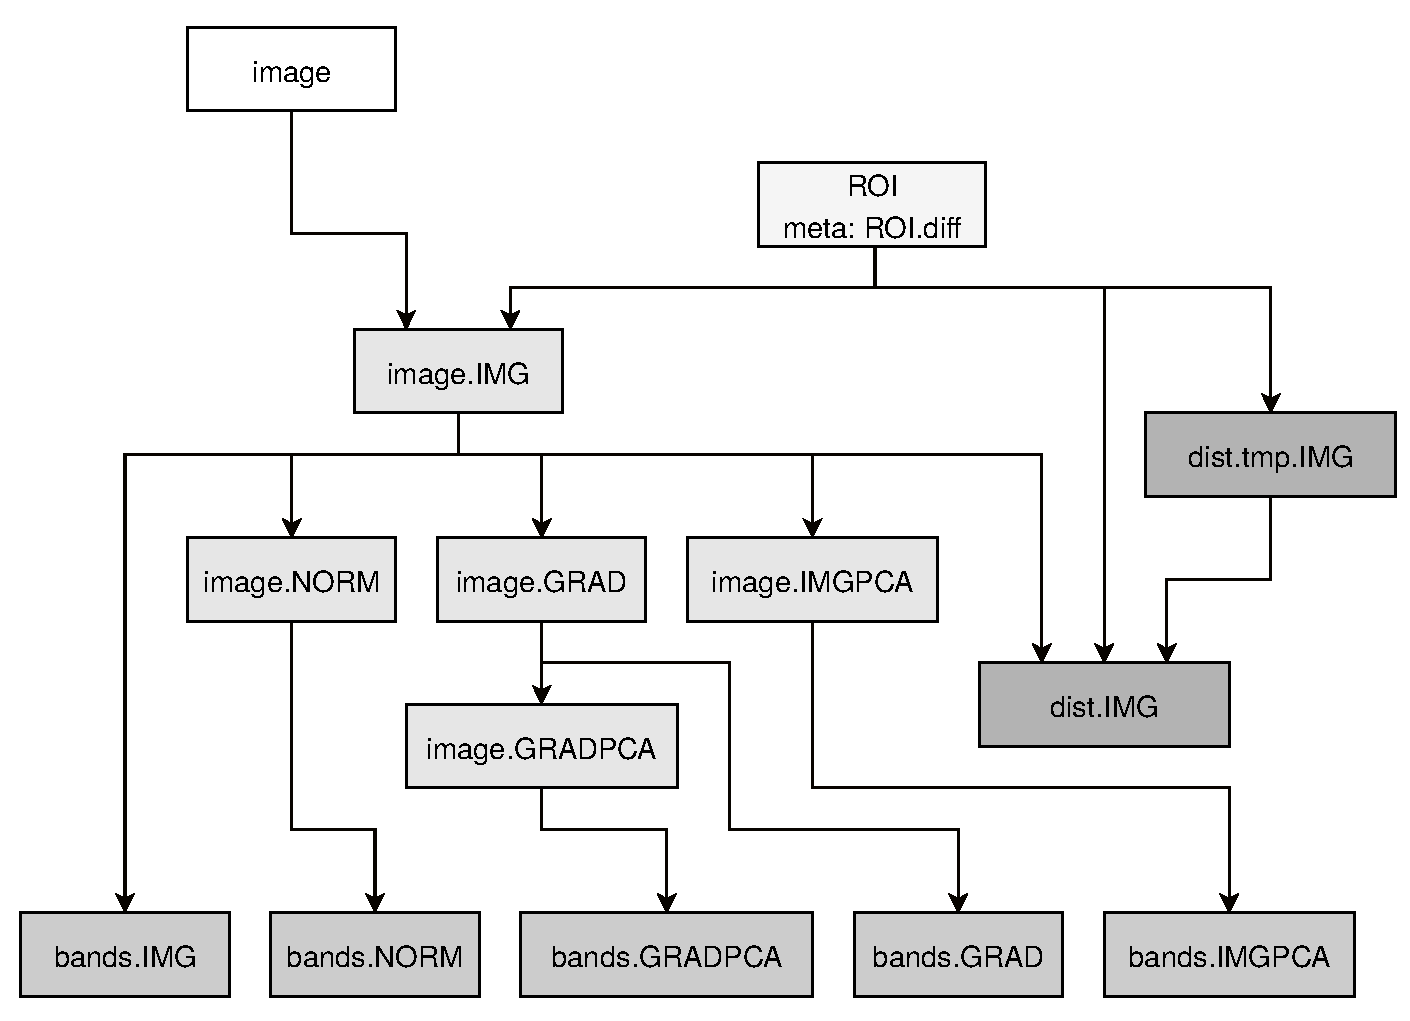
\includegraphics[width=0.7\linewidth]{rys02/data-dependencies}
	\caption{Graf zależności danych w systemie Gerbil}
	\label{fig:data-dependencies}	
\end{figure}

%\todo{Groty strzałek prawdopodobnie powinny być skierowane przeciwnie}
%\todo{Pojawiają się dziwne problemy z wstawieniem tego obrazka}

Na rysunku ~\ref{fig:data-dependencies} przedstawiono diagram zależności danych. Dane jednego koloru są do siebie semantycznie zbliżone. Przykładowo, image.NORM, image.GRAD, image.GRADPCA itp. są reprezentacjami obrazu oryginalnego. Dane posiadają również swoje metadane. Przykładowo metadaną ROI jest ROI.diff, które określa różnicę pomiędzy aktualnym a~poprzednim ROI. 

\subsection{Wpływ hierarchii danych na proces wykonania}
Analizując rysunek ~\ref{fig:data-dependencies} można dojść do wniosku, że proces przetworzenia danych jest dyktowany poprzez ich hierarchię. Przykładowo do obliczenia image.GRADPCA wymagane jest aby dane image, ROI, image.IMG oraz image.GRAD były już przetworzone. Dodatkowo można określić porządek, w którym te dane powinny zostać obliczone:

\begin{enumerate}[labelwidth=\widthof{\ref{last-item}},label=\arabic*.]
	\item image (podczas inicjalizacji systemu),
	\item ROI,
	\item image.IMG,
	\item image.GRAD,
	\item image.GRADPCA. \label{last-item}
\end{enumerate}

Scenariusz ten zakłada obliczenie każdej danej w hierarchii, co jest przypadkiem skrajnym. Często zdarza się, że pewna część danych jest aktualna. Wówczas przetwarzanie powinno rozpocząć się od pierwszej nieaktualnej danej znajdującej się najwyżej w hierarchii. 

Dodatkowo należy rozpatrzeć scenariusz równoległego wykonywania zadań. Zakładając, że aplikacja wyświetla jednocześnie dane image.NORM oraz image.GRAD, natomiast image.IMG zostało odświeżone, można dojść do wniosku, że system powinien w następnym kroku dokonać obliczeń obu danych (image.NORM i~image.GRAD). Obliczenia te można wykonać szeregowo bądź równolegle, wobec tego można zdefiniować opcjonalne wymaganie dla systemu zarządzania zadaniami jako możliwość równoległego przetwarzania zadań.
